% Chapter Template

\chapter{Methodology} % Main chapter title
\label{chapter3} 

The following chapter includes methodological procedures that are common for all chapters.
More detailed methodological procedures will be described in each chapter separately. 

\section{Data}
\label{ssec:data}
We already briefly presented the datasets in the first chapter in Section \ref{sec:data}.
Here, we will do an in-depth presentation of the datasets and present how we processed and cleaned the data. 

\subsection{Non-Intrusive Load Monitoring (NILM)}

While the NILM method was described in Chapter \ref{chapter2}, we will reintroduce it as part of the methodology.
NILM is a method that enables us to disaggregate consumption patterns of the whole building from a single meter.
The conventional method would be to meter installed for each consumer.
An alternative would be NILM. With this method, one meter can be used to find out which appliances consume the most energy.

The data used here was collected for means of research we did on Non-Intrusive load Monitoring (NILM) in publication \cite{Blaz2022}.
Where we used this data to perform a classification of appliances using deep learning.
Using Gramian angular fields (GAF) we transform time series into images.
We used multiple images in series to form a stack, a video.
Using deep learning architecture utilizing LSTM that used a stack of images as input, we were able to classify appliances with an F1 score of 80 \%.
Such techniques could be used to recognize appliances in unlabeled datasets, or help find possible mislabeling in existing datasets.

\subsection{Dataset Selection}

The Table \ref{tab:other_datasets} was published on the NILMTK \cite{nilmtk} wiki page. 
NILMTK is a tool developed by authors in paper \cite{nilmtk}.
It intends to make the development of NILM algorithms easier by standardizing a format in which building energy consumption datasets are stored. 
They also developed converters to convert existing datasets into a universal format.

This enables engineers to simply load and process multiple datasets.
NILMTK includes a dataset converter from most of the datasets from Table \ref{tab:other_datasets}.
\begin{table}[H]
    \caption{List of NILM datasets.}
    \centering
    \resizebox{\textwidth}{!}{\begin{tabular}{|l|l|l|l|l|l|l|l|l|}
    \hline
        \textbf{Dataset} & \textbf{Sampling rate} & \textbf{Duration } & \textbf{ Buildings } & \textbf{Subject} & \textbf{Country} & \textbf{Availability} \\ \hline
        Dataport & 1 Hz to 1 minute & 4+ years & 1200 & multiple & US & Licensed \\ \hline
        BLOND-50  & 50 kHz/6.4kHz & 213 days & 1 & office & Germany & Public \\ \hline
        FIRED & 12 kHz to 1 Hz & 101 days & 1 & residential & Germany & Public \\ \hline
        REDD & 16500 Hz / 1 Hz & 100 days & 5 & Residential & US & Request access \\ \hline
        BLUED & 12000 Hz & 7 days & 1 & Residential & US & Request access \\ \hline
        UK-DALE & 16000 Hz / 1 Hz & 2 years & 6 & Residential & UK & Public \\ \hline
        PLAID & 30000 Hz & 5 seconds & 55 & Appliances & US & Public \\ \hline
        WHITED & 44000 Hz & 5 seconds & 9 & Appliances & Multiple & Public \\ \hline
        Tracebase & 1 Hz & 1 day & 158 & Appliances & Germany & Request access \\ \hline
        DRED & 1 Hz / 1 min & 150 days & 1 & Residential & Netherlands & Public \\ \hline
        AMPds & 1 minute & 2 years & 1 & Residential & Canada & Public \\ \hline
        RAE & 1 Hz & 72 days & 1 & Residential & Canada & Public \\ \hline
        iAWE & 1 Hz & 73 days & 1 & Residential & India & Public \\ \hline
        HES & 2 minutes & 1 year & 251 & Residential & UK & Request access \\ \hline
        REFIT & 8 seconds & 2 years & 20 & Residential & UK & Public \\ \hline
        ECO & 1 second & 200 days & 6 & Residential & Switzerland & Public \\ \hline
        COMBED & 30 seconds & 30 days & ~ & Office & India & ~ \\ \hline
        IHEPCDS & 1 minute & 4 years & 1 & ~ & France & ~ \\ \hline
        SMART & 1 Hz & 60 days & 3 & ~ & USA & ~ \\ \hline
        LIT-Dataset & 15 kHz & 30 seconds & 26 & Residential & Brazil & Public \\ \hline
    \end{tabular}}
    \par 
    \par\footnotesize{Pruned version of the Table published by authors on NILMTK\protect{\cite{nilmtk}} wiki page. Full table available here \protect{\url{https://web.archive.org/web/20190607094329/http://wiki.nilm.eu/datasets.html}}.}
    \label{tab:other_datasets}
\end{table}



The reason why more datasets were not selected from the Table \ref{tab:other_datasets},
was because we followed the criteria:
\begin{enumerate}
    \item Sampling rate between 1 Hz and 1/10 Hz
    \item Duration more than 30 days
    \item Subject had to be a residential area building
    \item Include main meter as well as sub-meter measurements
    \item Has to be accessible
\end{enumerate}

After applying these criteria we were left with the following datasets:

\begin{itemize}
    \item UK-DALE \cite{UKDALE}
    \item REFIT \cite{REFIT}
    \item ECO \cite{ECO}
    \item REDD \cite{REDD}
    \item iAWE \cite{iAWE}.
\end{itemize}

While the Dataport dataset seems to be the best fit and of the best quality, it did sadly not meet our criteria as it is a closed dataset available only via license.

\subsection{Processing}

After datasets were obtained and converted they were ready to be processed.
We decided to slice the data into hourly slices so that it will be easier to find missing data and build LPs.

Firstly we resampled the time series data  1/6 Hz. 
This had to be done since datasets were sampled at different frequencies.
A frequency of 1/6 Hz is commonly used since it has a good ratio between resource usage and NILM algorithm performance.
Resampling was done using Pandas resample. 
We used a forward fill parameter with a limit of 5.
This means that in case of missing data, we will fill in no more than 5 samples with the last known value.
Secondly, we sliced the time series data into hourly slices. 
One sample every 6 seconds means, there were roughly 60 samples in every slice.
Thirdly, we removed slices with missing data.
This was done for all slices where there was more than 20 \% of data missing.
In cases where less than 20 \% of data were missing, we forward-filled it with the last known value.
In the worst case, we forward filled 12 samples. 
Finally, resampled and cleaned data was stored in the .hdf file.
% \begin{verbatim}
%    /dataset/appliance/building/cleaned_dataset
% \end{verbatim}
% This hierarchical way of storing the data enabled us to encode labels into the sub-dataset path.
% In the end, there was sub-dataset for every appliance for every building for every dataset.


\subsection{Splitting and Evaluation} \label{ssec:ds_eval}

In some cases, datasets had to be split, so that the algorithm we developed in Chapter \ref{chapter6}, may be empirically evaluated. 
The data was split into train and test sets, where 80 \% of the data was used for training and 20 \% percent of the data for testing.
The data was split based on the number of samples, so in some cases where there is a lot of missing data, the time window of test data might be longer, although it contains only 20 \% of the samples.

\subsection{Dataset analysis}
Table \ref{tab:dataset_analysis} presents all 5 datasets that we have made use of.
The second column shows the number of samples for each dataset.
Numbers can be a bit deceptive when it comes to the actual amount since data was resampled.
To confront this, a third column was created.
Here we present the actual number of samples,
that is number that was obtained after resampling.
We also divided the number of samples by $10^6$, to make the column comprehensible.

% \begin{table}[H]
%     \centering
%     \begin{tabular}{|l|r|r|r|}
%     \hline
%     \textbf{Dataset} & \multicolumn{1}{l|}{\textbf{Samples}} & \multicolumn{1}{l|}{\textbf{Resampled*10\textasciicircum{}-6}} & \multicolumn{1}{l|}{\textbf{Buildings}} \\ \hline
%     REFIT            & 144341850                             & 192.46                                                         & 20                                      \\ \hline
%     UK-DALE          & 54997820                              & 55                                                             & 5                                       \\ \hline
%     ECO              & 130187888                             & 21.7                                                           & 6                                       \\ \hline
%     iAWE             & 6425055                               & 6.43                                                           & 1                                       \\ \hline
%     REDD             & 5890953                               & 5.89                                                           & 6                                       \\ \hline
%     \end{tabular}
%     \caption{Appliances sorted by number of samples for REFIT}
%     \label{tab:dataset_analysis}
% \end{table}

\begin{table}[H]
    \caption{Summary of datasets and their characteristics}
    \centering
    \begin{tabular}{lrrr}
        \toprule
        \textbf{Dataset} & \textbf{Samples (M)} & \textbf{Buildings} \\
        \midrule
        REFIT   &   192.46 & 20 \\
        UK-DALE &   55     &  5 \\
        ECO     &   21.7   &  6 \\
        iAWE    &   6.43   &  1 \\
        REDD    &   5.89   &  6 \\
        \bottomrule
    \end{tabular}
    \label{tab:dataset_analysis}
    \par\footnotesize{Note: Samples are abbreviated as M for millions.}
\end{table}

The figures below show where time splits between train and test data were done.
At the same time, we can also observe the health of each dataset.
By healthy dataset, we presume a dataset that has a long uninterrupted timeline with many buildings.


\subsubsection{REFIT}
The REFIT \cite{REFIT} dataset included data for more than 15 buildings, as can be seen in the Figure below.
The dataset in general is of the highest quality since it is the longest with the least missing data.
This means this dataset should give the most relevant results.
\begin{figure}[H]
	\centering
	\caption{Timeline for REFIT}
	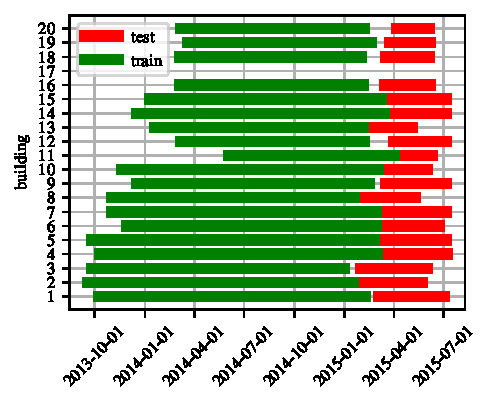
\includegraphics[]{Figures/EC/refit_timeline.pdf}
	\label{fig:refit_timeline}
\end{figure}

Figure \ref{tab:refit_table} presents appliances sorted by a number of samples, where the top 10 were selected.
Together, REFIT contains data for 23 different appliances from 20 homes.

% \begin{table}[H]
%     \centering
%     \begin{tabular}{|l|r|r|r|}
%     \hline
%     \textbf{Appliances} & \multicolumn{1}{l|}{\textbf{Instances}} & \multicolumn{1}{l|}{\textbf{Samples}} & \multicolumn{1}{l|}{\textbf{Resampled*10\textasciicircum{}-6}} \\ \hline
%     fridge freezer      & 15                                      & 35392570                              & 47.19                                                        \\ \hline
%     television          & 20                                      & 30104492                              & 40.14                                                         \\ \hline
%     freezer             & 13                                      & 28430845                              & 37.91                                                        \\ \hline
%     computer            & 12                                      & 13529700                              & 18.04                                                        \\ \hline
%     fridge              & 7                                       & 9132793                               & 12.18                                                        \\ \hline
%     dishwasher          & 15                                      & 4275136                               & 5.7                                                         \\ \hline
%     washing machine     & 20                                      & 4189799                               & 5.59                                                         \\ \hline
%     microwave           & 17                                      & 4119921                               & 5.49                                                         \\ \hline
%     pond pump           & 1                                       & 3284418                               & 4.38                                                         \\ \hline
%     broadband router    & 2                                       & 2134626                               & 2.85                                                         \\ \hline
%     \end{tabular}
%     \caption{Appliances sorted by number of samples for REFIT}
%     \label{tab:refit_table}
% \end{table}

\begin{table}[H]
    \centering
    \caption{Appliances sorted by number of samples for REFIT}
    \label{tab:refit_table}
    \begin{tabular}{@{}lrrr@{}}
        \toprule
        \textbf{Appliances} & \textbf{Instances}  & \textbf{Samples (M)} \\
        \midrule
        fridge freezer      & 15           & 47.19                \\
        television          & 20           & 40.14                \\
        freezer             & 13           & 37.91                \\
        computer            & 12           & 18.04                \\
        fridge              & 7            & 12.18                \\
        dishwasher          & 15           & 5.70                 \\
        washing machine     & 20           & 5.59                 \\
        microwave           & 17           & 5.49                 \\
        pond pump           & 1            & 4.38                 \\
        broadband router    & 2            & 2.85                 \\
        \bottomrule
    \end{tabular}
    \par\smallskip
    \footnotesize{Note: Samples are abbreviated in millions as M.}
\end{table}


\subsubsection{UK-DALE} 

Through the UK-DALE \cite{UKDALE} dataset is of similar size, most of the data is from building 1.
In general, it includes 5 years of data, but only for some appliances, where many appliances are rarely used.
When taking all of this into account, there were too many issues with building 1, and it was simply ignored.
Another issue that can be seen in Figure \ref{fig:ukdale_timeline} is that there is not enough data for 
building 3. The test includes only a week of data, which is not enough for representative results, therefore it was ignored.
The rest of the buildings seem healthy.

\begin{figure}[H]
	\centering
	\caption{Timeline for UK-DALE}
	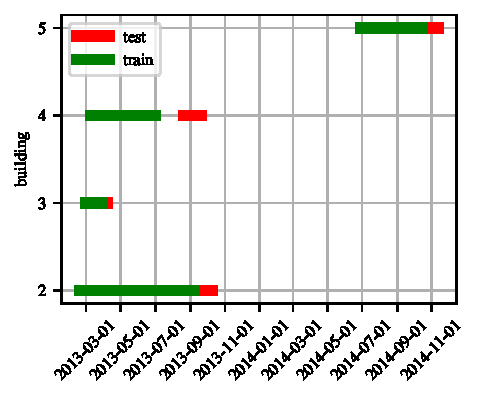
\includegraphics[]{Figures/EC/ukdale_timeline.pdf}
	\label{fig:ukdale_timeline}
\end{figure}

Figure \ref{tab:ukdale_table} presents appliances sorted by a number of samples, where top 10 were selected.
Together, UKDALE contains data for 53 different appliances.

% \begin{table}[H]
%     \centering
%     \begin{tabular}{|l|r|r|r|}
%     \hline
%     \textbf{Appliances}           & \multicolumn{1}{l|}{\textbf{Instances}} & \multicolumn{1}{l|}{\textbf{Samples}} & \multicolumn{1}{l|}{\textbf{Resampled*10\textasciicircum{}-6}} \\ \hline
%     light                         & 15                                      & 9861973                               & 9.86                                                         \\ \hline
%     fridge freezer                & 2                                       & 8830004                               & 8.83                                                         \\ \hline
%     HTPC                          & 1                                       & 4867154                               & 4.87                                                         \\ \hline
%     solar thermal pumping station & 1                                       & 4254460                               & 4.25                                                         \\ \hline
%     audio amplifier               & 2                                       & 3996912                               & 4                                                            \\ \hline
%     boiler                        & 2                                       & 3753032                               & 3.75                                                         \\ \hline
%     computer monitor              & 4                                       & 3203552                               & 3.2                                                          \\ \hline
%     television                    & 3                                       & 2590025                               & 2.59                                                         \\ \hline
%     desktop computer              & 3                                       & 2551053                               & 2.55                                                         \\ \hline
%     laptop computer               & 4                                       & 2099697                               & 2.1                                                          \\ \hline
%     microwave                     & 3                                       & 1804223                               & 1.8                                                          \\ \hline
%     \end{tabular}
%     \caption{Appliances sorted by number of samples for UK-DALE}
%     \label{tab:ukdale_table}
% \end{table}

\begin{table}[H]
    \caption{Summary of datasets and their characteristics}
    \centering
    \begin{tabular}{lrr}
        \toprule
        \textbf{Appliances}           & \textbf{Instances} & \textbf{Samples (M)} \\
        \midrule
        light                         & 15                 & 9.86                                  \\
        fridge freezer                & 2                  & 8.83                                  \\
        HTPC                          & 1                  & 4.87                                  \\
        solar thermal pumping station & 1                  & 4.25                                  \\
        audio amplifier               & 2                  & 4                                     \\
        boiler                        & 2                  & 3.75                                  \\
        computer monitor              & 4                  & 3.2                                   \\
        television                    & 3                  & 2.59                                  \\
        desktop computer              & 3                  & 2.55                                  \\
        laptop computer               & 4                  & 2.1                                   \\
        microwave                     & 3                  & 1.8                                   \\
        \bottomrule
    \end{tabular}
    \label{tab:ukdale_table}
\end{table}


\subsubsection{ECO}
ECO \cite{ECO} dataset has a length of data similar to UK-DALE. 
The only issue is building 1, where there is a lot of missing data.
This is a good example of how data is split, it is split based on several samples,
meaning that there is 80 \% in the train bar, due to missing data the second bar is longer. 

\begin{figure}[H]
	\centering
	\caption{Timeline for ECO}
	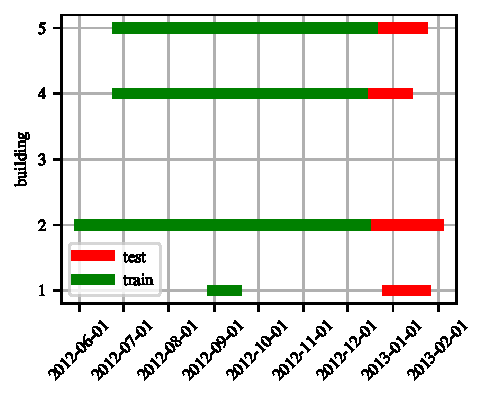
\includegraphics[]{Figures/EC/eco_timeline.pdf}
	\label{fig:eco_timeline}
\end{figure}

Table \ref{tab:eco_table} shows that there were a lot of samples for the ECO dataset.
This number was reduced by a factor of 6 after resampling was done.

% \begin{table}[H]
%     \centering
%     \begin{tabular}{|l|r|r|r|}
%     \hline
%     \textbf{Appliances} & \multicolumn{1}{l|}{\textbf{Instances}} & \multicolumn{1}{l|}{\textbf{Samples}} & \multicolumn{1}{l|}{\textbf{Resampled*10\textasciicircum{}-6}} \\ \hline
%     freezer             & 4                                       & 33464965                              & 5.58                                                        \\ \hline
%     fridge              & 6                                       & 25532449                              & 4.26                                                        \\ \hline
%     computer            & 3                                       & 16122644                              & 2.69                                                        \\ \hline
%     HTPC                & 5                                       & 15647899                              & 2.61                                                        \\ \hline
%     audio system        & 1                                       & 5891389                               & 0.98                                                         \\ \hline
%     laptop computer     & 5                                       & 5073161                               & 0.85                                                         \\ \hline
%     television          & 1                                       & 4182306                               & 0.7                                                         \\ \hline
%     lamp                & 3                                       & 3361625                               & 0.56                                                         \\ \hline
%     broadband router    & 1                                       & 1778507                               & 0.16                                                         \\ \hline
%     washing machine     & 1                                       & 972600                                & 0.12                                                         \\ \hline
%     \end{tabular}
%     \caption{Appliances sorted by number of samples for ECO}
%     \label{tab:eco_table}
% \end{table}

\begin{table}[H]
    \centering
    \begin{tabular}{lrrr}
        \toprule
        \textbf{Appliances} & \textbf{Instances} & \textbf{Samples (M)}  \\
        \midrule
        freezer             & 4                   & 5.58                 \\
        fridge              & 6                   & 4.26                 \\
        computer            & 3                   & 2.69                 \\
        HTPC                & 5                   & 2.61                 \\
        audio system        & 1                   & 0.98                 \\
        laptop computer     & 5                   & 0.85                 \\
        television          & 1                   & 0.70                 \\
        lamp                & 3                   & 0.56                 \\
        broadband router    & 1                   & 0.16                 \\
        washing machine     & 1                   & 0.12                 \\
        \bottomrule
    \end{tabular}
    \caption{Summary of appliances in the ECO dataset}
    \label{tab:eco_table}
\end{table}


\section{Activation Detection}

How appliance activations are extracted was already mentioned in Subsection \ref{ssec:feature_set}.
There we said, the activation occurs when consumption exceeds $P_{thr}$.
This is portrayed in Figure \ref{fig:sig_proc_fig} in the same subsection.

This threshold was selected as the standard value of 10 W.
This value is used as a standard threshold in NILMTK \cite{nilmtk}.

This hard-set value is an issue for appliances that consume small amounts of energy,
but still, show interesting usage patterns.
One such example would be a mobile phone charger or broadband router.
Issues could occur even with larger consumers such as smart TVs, that could consume more than 10W even when they are not operating.

In order to check that this was not an issue we came up with a test.
We created a histogram of power values, with a resolution of 10 W, where one such example can be seen in Figure \ref{fig:freq_pthr}.
For appliances that are mostly off, the first bucket should be the most populated.
This was true for the majority of appliances and with that, they passed the test.
For the ones that this was not true, we manually checked them and were either discarded or given a new threshold.
The new threshold was manually set between the first and the second frequency peak. 

\begin{figure}[H]
	\centering
	\caption{Histogram of power values for Toaster}
	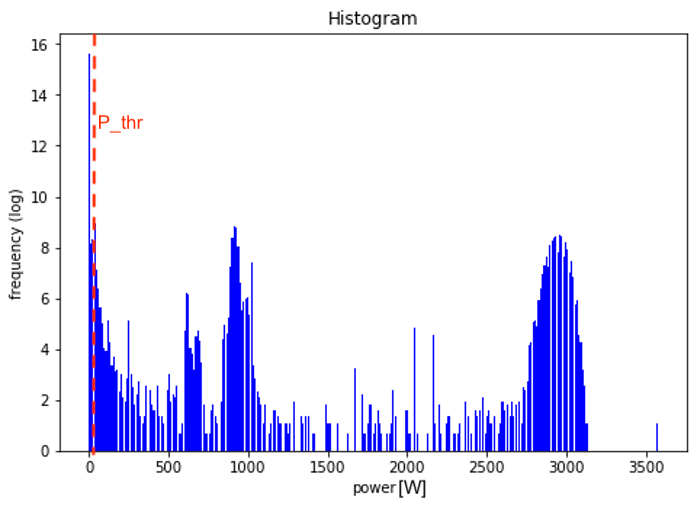
\includegraphics[width=0.9\textwidth]{Figures/profile_sketches/freq_pthr.png}
	\label{fig:freq_pthr}
\end{figure}

When we are observing Figure \ref{fig:freq_pthr}, we have to keep in mind that the frequency scale is logarithmic.
Another thing to note is, that Figure \ref{fig:freq_pthr} is also an LP, that we mention expanded table of LPs in Appendix \ref{AppendixB}.
This LP is useful for the detection operation modes.
In this case, we can see that this Toaster has three operating modes, where each peak is a unique mode.
One at 3 kW, the second at 1 kW and the third at 0.7 kW.
Setting thresholds around these peaks could enable us to build 3 different LPs, where each one would present a different usage pattern.

\section{Infrastructure and Software Used}

To process the data and to obtain the results the environment and virtual machines from Google Colab \cite{colab} were used.
They offer access to Google GPU-accelerated compute machines with 12 GB of RAM. 
Colab also offers access to Drive cloud storage, where the dataset and results were stored.
While running the experiments, we made use of Drives 100 TB pooled cloud storage, which is available to students of the University of Ljubljana. 
For development and version control, GitHub was used. 

Within the Colab which uses a Jupyter \cite{jupyter} environment at its core, various python libraries were used.
To store and read the datasets in hdf5 format we used h5py  \cite{hdf5} and Pickle  \cite{pickle}.
To load datasets into RAM and then handle them, the pandas  \cite{pandas} library was used.
For handling the large matrices and calculating we used NumPy  \cite{numpy}.
To present the data with graphs we have used Matplotlib  \cite{matplotlib} and to present data with heatmap Seaborn  \cite{seaborn}.
For easier implementation, such as of the t-SNE, a Scikit  \cite{scikit} and SciPy  \cite{scipy} libraries were used.
